% vim: set tw=0:
\documentclass{beamer}
\usepackage{graphicx}
\usepackage{hyperref}
\hypersetup{pdfborder={0 0 0 0}}

% Reasonable themes:
% Antibes Bergen Berkeley Berlin Frankfurt Goettingen Ilmenau Luebeck Malmoe
% Montpellier PaloAlto Rochester Singapore Szeged Warsaw bars boxes
% compatibility default lined plain shadow sidebar split tree
% And these ones include the author's name on every slide:
% Berkeley

% Declare themes.
\mode<presentation>
\usetheme{UWHEP}

% Personal macros.
\newcommand{\email}[1]{{\texttt #1}}
\newcommand{\newframe}[1]{\section{#1}
    \frametitle{\sc{#1}}}
\newcommand{\subframe}[1]{\subsection{#1}
    \frametitle{\sc{#1}}}
\newcommand{\supers}[1]{\ensuremath{^\textrm{#1}}}
\newcommand{\subs}[1]{\ensuremath{_\textrm{#1}}}
\newcommand{\ca}{\ensuremath{\sim}}
\renewcommand{\email}[1]{\href{mailto:#1}{\nolinkurl{#1}}}

% Author information.
\title{T2 Status}
\author[Maier, Mohapatra]{
    Will Maier \and Ajit Mohapatra\\ 
    {\tt wcmaier@hep.wisc.edu}\\
    {\tt ajit@hep.wisc.edu}}
\institute[Wisconsin]{University of Wisconsin - High Energy Physics}
\date{2009.09.01}
\logo{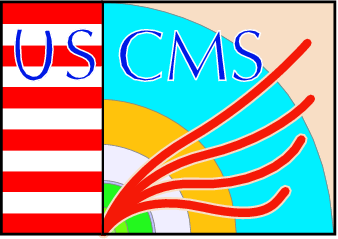
\includegraphics[height=0.6cm]{../../../Graphics/USCMS_logo.png}\hspace{.1cm}
\includegraphics[height=0.75cm]{../../../Graphics/UW_logo.png}}

\begin{document}

\begin{frame}
    \titlepage
\end{frame}

%\section{Overview}
%\begin{frame}
%    \tableofcontents
%\end{frame}

\section{Facilities}
\subsection{Software and Storage}
\begin{frame}
\frametitle{}

\begin{itemize}
	\item SL5 on most resources
	\begin{itemize}
		\item Upgrading some dCache pools is slower, because root disks also have some pool data
	\end{itemize}
	\item Built new systems infrastructure (Yum, Cfengine, Kickstart)
	\item Integrated key SL4 systems with new infrastructure and applied all outstanding errata
	\begin{itemize}
		\item Future updates on a regular schedule
	\end{itemize}
	\item Switch stack failed 2009.08.23; bug in old IOS
	\item Moving to campus management of network on 2009.09.02
	\begin{itemize}
		\item Better monitoring/planning for future expansion
		\item Better management of switches (including software updates)
		\item Eliminate bottlenecks between newer compute/storage resources
	\end{itemize}
	\item Increased dcap limits again
\end{itemize}

\end{frame}

\subsection{Production and Monitoring}
\begin{frame}
\frametitle{}
\begin{itemize}
	\item JobRobot: OK
	\item SAM: Monitoring blip due to switch failure and dcap limits 2009.08.21-23
	\item RSV: OK
	\item PhEDEx:
	\begin{itemize}
		\item Still running 3\_2\_0; will upgrade to 3\_2\_1 sometime this week
		\item Uplinks from Wisconsin are commissioned to all the remaining T1s
		\item Usual MC transfers for local users
	\end{itemize}
	\item MC Production:
	\begin{itemize}
		\item FDMC and FAMC @ 10TeV are complete (total 288M in less than a month)
		\item FDMC @ 7TeV (112M for now) running
		\item Performance in OSG is good.
		\item Omaha has recovered from downtime and production is resuming there
		\item So far only one local DBS instance for MC production; another will be added for local users once our new DB server is up
	\end{itemize}
\end{itemize}
\end{frame}

\end{document}
